% Protocol-Governed Systems: A Constitutional Realization of Turing-Complete Systems
% arXiv-compatible single-column format
\documentclass[11pt,a4paper]{article}

% Standard packages for arXiv compatibility
\usepackage[utf8]{inputenc}
\usepackage[T1]{fontenc}
\usepackage{lmodern}
\usepackage{amsmath,amssymb,amsthm}
\usepackage{graphicx}
\usepackage{hyperref}
\usepackage[margin=1in]{geometry}
\usepackage{natbib}
\usepackage{booktabs}
\usepackage{tikz}
\usetikzlibrary{shapes,arrows,positioning,calc,fit,backgrounds,decorations.pathreplacing}
\usepackage{enumitem}
\usepackage{microtype}
\usepackage{xcolor}
\usepackage{float}

% Allow more flexibility in line breaking to avoid overfull hboxes
\emergencystretch=2em

% Color definitions for figures
\definecolor{classicalcolor}{RGB}{234,67,53}
\definecolor{governedcolor}{RGB}{52,168,83}
\definecolor{sharedcolor}{RGB}{66,133,244}
\definecolor{layerlight}{RGB}{232,240,254}
\definecolor{turingcolor}{RGB}{180,167,214}
\definecolor{lambdacolor}{RGB}{147,196,125}
\definecolor{registercolor}{RGB}{246,178,107}
\definecolor{protocolcolor}{RGB}{109,158,235}

% Hyperref setup
\hypersetup{
    colorlinks=true,
    linkcolor=blue,
    citecolor=blue,
    urlcolor=blue
}

% Theorem environments
\newtheorem{theorem}{Theorem}
\newtheorem{proposition}{Proposition}
\newtheorem{definition}{Definition}

\title{Protocol-Governed Systems:\\A Constitutional Realization of Turing-Complete Systems}

\author{Bachi (aka Bhash Ganti)\\
\texttt{bachi.bachi@myyahoo.com}}

\date{}

\begin{document}

\maketitle

\begin{abstract}
Modern discussions of Turing completeness focus on the expressive power of programming languages or virtual machines. Such treatments implicitly assume imperative control flow, mutable state, and unconstrained execution semantics. This paper presents an alternative formulation: a protocol-governed computational system that is Turing complete by construction, while remaining constitutionally bounded, auditable, and behaviorally deterministic.

Building on prior work introducing protocol-governed software architecture \citep{bachi2026protocol}, we demonstrate that general computation can be realized through declarative behavioral artifacts interpreted by a semantically blind execution engine. Computation emerges from the lawful composition of protocol primitives---pure transforms, governed side effects, and workflow orchestration---rather than from imperative code paths.

We formalize the conditions under which protocol-governed systems satisfy the requirements of universal computation, while simultaneously constraining execution through governance, traceability, and explicit authority boundaries. Unlike traditional Turing machines, whose power derives from unconstrained state mutation and control flow, protocol-governed computation achieves expressiveness through controlled composition and explicit semantics.

This work reframes Turing completeness as an architectural property rather than a language feature, and argues that protocol-governed computation offers a viable foundation for high-assurance, AI-era systems where execution must remain auditable, deterministic, and evolution-resilient.
\end{abstract}

\noindent\textbf{Categories:} Software Engineering (cs.SE), Programming Languages (cs.PL), Computational Complexity (cs.CC)

\noindent\textbf{Keywords:} Turing completeness, universal computation, protocol governance, declarative systems, constitutional architecture, deterministic execution, auditability, AI-era software


%% ============================================================
%% SECTION 1: INTRODUCTION
%% ============================================================

\section{Introduction}
\label{sec:introduction}

\subsection{Motivation: Why Turing Completeness Is No Longer Enough}

The theory of computation has long celebrated Turing completeness as the definitive measure of computational power. A system is deemed ``complete'' if it can simulate any Turing machine---if it can compute any function that is computable in principle \citep{turing1936computable}. This criterion, established nearly a century ago, remains the benchmark against which programming languages, virtual machines, and computational models are evaluated.

Yet Turing completeness, as classically formulated, is silent on questions that dominate contemporary software engineering. It says nothing about \emph{governance}---who may authorize computation and under what constraints. It says nothing about \emph{auditability}---whether execution can be inspected, replayed, or verified. It says nothing about \emph{semantic stability}---whether a system's meaning can be preserved as its implementation evolves.

These omissions were tolerable when computation was a scarce resource, carefully managed by human programmers who understood both intent and implementation. They become intolerable in the AI era, where large language models generate code at velocities that exceed human capacity to audit \citep{chen2021evaluating}. When AI produces the majority of production software---a transition industry analysts project within this decade \citep{github2023copilot}---the question shifts from ``Can this system compute?'' to ``Can this system be governed?''

A system may be Turing complete and yet ungovernable: its behavior implicit, its side effects unbounded, its execution irreproducible. Such systems pose existential risks in domains requiring regulatory compliance, financial accountability, or safety-critical operation. The classical criterion of computational universality provides no protection.

This paper argues that Turing completeness must be reconceived---not abandoned, but reframed. We seek systems that are \emph{universally expressive} yet \emph{constitutionally constrained}: capable of computing any computable function while remaining bounded by explicit governance, traceable through observable execution, and resilient to semantic drift under implementation evolution.

\subsection{The Governance Deficit in Classical Computation Models}

Classical computational models---Turing machines, lambda calculus, register machines---share a characteristic that renders them unsuitable as foundations for governed systems: they are \emph{semantically unconstrained}.

A Turing machine's tape is infinite and arbitrarily mutable. Its transition function may encode any computable behavior. There is no authority that sanctions state changes, no trace that records execution history, no invariant that constrains permissible operations. The machine simply computes, and computation is its own justification.

This unconstrained expressiveness was precisely the point. Church, Turing, and their contemporaries sought to characterize the \emph{limits} of computation---what could and could not be computed in principle \citep{church1936unsolvable}. Governance was not merely absent from their models; it was deliberately excluded to achieve mathematical generality.

Modern systems inherit this unconstrained heritage. Programming languages, virtual machines, and execution runtimes provide Turing-complete expressiveness without governance mechanisms. Any behavior that is computable is permissible. Constraints, when they exist, are bolted on after the fact through static analysis, runtime monitoring, or procedural controls. These mechanisms inspect computation from the outside; they do not arise from computational architecture itself.

Protocol-governed systems take a different approach. Governance is not external to computation but constitutive of it. Behavioral constraints are not inspected after the fact but encoded in the very artifacts that define computable behavior. The question ``Is this computation permitted?'' has a structural answer, not a procedural one.

\subsection{Contribution Summary}

This paper makes three contributions to the foundations of governed computation:

\begin{enumerate}[nosep]
    \item \textbf{Architectural Reframing of Turing Completeness.} We demonstrate that Turing completeness can be realized as a property of protocol-governed architecture rather than a feature of programming languages. Universal computation emerges from declarative artifact composition, not imperative code execution.

    \item \textbf{Constitutionally Constrained Computation.} We introduce and formalize the concept of \emph{constitutionally constrained computation}: systems that achieve universal expressiveness while remaining bounded by explicit governance, traceable through execution observation, and resilient to semantic drift.

    \item \textbf{Governance as Architectural Primitive.} We argue that governance must be treated as a first-class architectural concern---not as an external constraint on computation but as an intrinsic property of computational systems. This reframing is essential for AI-era software where execution velocity exceeds human audit capacity.
\end{enumerate}


%% ============================================================
%% SECTION 2: BACKGROUND
%% ============================================================

\section{Background: Classical Models of Universal Computation}
\label{sec:background}

\subsection{The Turing Machine as Semantic Idealization}

Alan Turing's 1936 paper ``On Computable Numbers'' introduced the abstract machine that bears his name \citep{turing1936computable}. The Turing machine comprises an infinite tape divided into cells, a head that reads and writes symbols, a finite state register, and a transition function that determines head movement and symbol modification based on current state and symbol.

The power of the Turing machine lies in its universality. A universal Turing machine can simulate any other Turing machine given an encoding of that machine's transition function \citep{minsky1967computation}. This simulation capability establishes the machine as a model of general computation---a mathematical formalization of what it means to compute.

Yet the Turing machine is not a blueprint for governed computation. Its tape is infinite and unconstrained; any cell may be modified at any time. Its transition function is opaque; no external observer can determine why a state change occurred without simulating the entire computation. Its execution produces no trace; the only observable output is the final tape configuration (if the machine halts).

These properties were virtues for Turing's purpose: characterizing the theoretical limits of computation. They are deficits for our purpose: building systems whose behavior can be governed, audited, and preserved across implementation evolution.

\subsection{Modern Computational Descendants}

The Turing machine's descendants populate contemporary computing:

\textbf{Lambda Calculus.} Church's concurrent development of lambda calculus provides an equivalent model of computation based on function abstraction and application rather than state mutation \citep{church1936unsolvable,barendregt1984lambda}. Lambda calculus is computationally universal and foundational to functional programming. Yet it, too, is governance-silent: any lambda term may be constructed, and reduction proceeds without constraint.

\textbf{Register Machines.} Register machines model computation through finite registers and simple operations (increment, decrement, conditional branch) \citep{minsky1967computation,shepherdson1963computability}. They are closer to physical hardware than Turing machines while maintaining computational universality. Yet they inherit the same governance deficit: registers may be arbitrarily modified, and execution is unconstrained.

\textbf{Virtual Machines and Bytecode Runtimes.} Modern virtual machines (JVM, CLR, WASM) provide portable execution environments for compiled bytecode. They achieve practical universality within their instruction sets. Yet bytecode execution remains fundamentally unconstrained: any sequence of valid instructions may execute, and governance is external to the execution model.

\subsection{What Classical Models Omit}

Four concerns absent from classical computational models are central to governed systems:

\begin{description}[nosep]
    \item[Authority.] Classical models include no concept of authorization. Any computation that can be encoded can execute. There is no distinction between permitted and prohibited behavior at the model level.

    \item[Auditability.] Classical models produce no execution trace. The only observable artifact is the final result (if computation terminates). Intermediate states, decision points, and execution paths are invisible.

    \item[Deterministic Replay.] Classical models provide no mechanism for reproducing execution. Given the same program, different runs may produce different results due to non-determinism, timing dependencies, or external state.

    \item[Behavioral Traceability.] Classical models provide no mapping between execution events and declared behavioral intent. The ``why'' behind any state change must be inferred from code inspection, not observed from execution evidence.
\end{description}

These omissions are not accidents. They reflect the mathematical purpose of classical models: characterizing computability, not constraining it. A foundation for governed computation must address these concerns architecturally, not procedurally.


%% ============================================================
%% SECTION 3: PROTOCOL-GOVERNED EXECUTION
%% ============================================================

\section{Protocol-Governed Execution: A Different Starting Point}
\label{sec:protocol-governed}

\subsection{Separation of Behavior and Execution}

Protocol-governed systems begin from a fundamentally different architectural premise: the strict separation of \emph{what a system does} (behavior) from \emph{how it does it} (execution) \citep{ganti2024protocol}.

\textbf{Protocol artifacts} are declarative, version-controlled specifications that define permissible system behavior. They declare workflows, capability contracts, actor authorities, and state transitions in explicit, machine-readable form. Protocol artifacts are the constitutional law of the system---the authoritative specification against which all execution is measured.

\textbf{Execution engines} interpret protocol artifacts deterministically. They compile declarative specifications into executable structures, route operations to appropriate handlers, and produce traces that witness execution. Crucially, execution engines are \emph{semantically blind}: they have no knowledge of business domain meaning. They enforce protocol structure without understanding protocol semantics.

This separation enables a property unavailable in classical computational models: \emph{implementation replaceability}. Execution engines can be optimized, rewritten, or AI-generated without altering system behavior, provided they produce equivalent traces. Behavioral equivalence is verified mechanically through trace comparison, not through code review.

\subsection{Constitutional Constraints as First-Class}

In protocol-governed systems, constraints are not external to computation but constitutive of it:

\begin{description}[nosep]
    \item[Vocabulary-Bounded Behavior.] The protocol vocabulary defines the complete space of possible behaviors. Behaviors not expressible in the vocabulary cannot occur. This is not a limitation but a feature: the behavioral surface is explicitly bounded and auditable.

    \item[Explicit Side-Effect Surfaces.] All world-affecting operations are declared in capability contracts. There are no ambient side effects, no hidden mutations, no implicit external interactions. The system's risk profile is proportional to its declared side-effect surface.

    \item[Trace-Based Verification.] Every execution produces a structured trace that witnesses what occurred. Traces are the canonical evidence of system behavior---they enable replay, verification, and audit without implementation inspection.
\end{description}


%% ============================================================
%% SECTION 4: COMPUTATIONAL PRIMITIVES
%% ============================================================

\section{Computational Primitives in a Protocol-Governed System}
\label{sec:primitives}

Protocol-governed computation rests on four architectural primitives that collectively enable universal expressiveness while preserving governance. These primitives are described at the semantic level, without reference to specific encodings or implementation mechanisms.

\subsection{State Representation}

\textbf{Classical Model:} The Turing machine's infinite tape provides unbounded, arbitrarily-mutable storage. Any cell may be read or written at any time. State mutation is the fundamental computational act.

\textbf{Protocol-Governed Model:} State exists as protocol-declared artifacts and governed side effects. State transitions occur only through explicitly declared capability side effects. There is no ambient mutable memory---all storage is named, versioned, and traced.

The key distinction is \emph{explicitness}. In classical models, state is implicit infrastructure. In protocol-governed models, state is declared behavioral surface. Every state container has a name, a governance contract, and a modification trace.

This explicitness does not reduce expressiveness. Any state structure that can be represented on a Turing tape can be represented in governed storage. The difference is that governed storage maintains provenance: who authorized the state, when it changed, and through what protocol operation.

\subsection{Control Flow}

\textbf{Classical Model:} Turing machines and their descendants achieve control flow through transition functions, conditional branches, and unbounded loops. Control can jump to any reachable state.

\textbf{Protocol-Governed Model:} Control flow is expressed through declarative workflow orchestration. Workflows define directed acyclic graphs of operations, with branching expressed as conditional node routing rather than imperative jumps.

The question arises: can acyclic workflow structures express the unbounded iteration required for Turing completeness? The answer is yes, through \emph{lawful re-invocation}. A workflow may invoke another workflow, including (through versioning) workflows that achieve equivalent behavioral recursion. The recursion is not lexical but semantic: it occurs through protocol-declared invocation paths, not through goto-equivalent jumps.

\subsection{Computation}

\textbf{Classical Model:} Computation occurs through primitive operations on state---symbol writes on the Turing tape, beta reductions in lambda calculus, register modifications in register machines.

\textbf{Protocol-Governed Model:} Computation occurs through \emph{capability transforms}: pure, deterministic functions that accept declared inputs and produce declared outputs. Transforms have no side effects; they are replayable, cacheable, and compositional.

Expressiveness emerges through \emph{composition}. Complex computations assemble from primitive transforms through workflow orchestration. Each transform is independently testable and governable. The composition itself is declared in protocol artifacts, not implicit in code structure.

\subsection{Observation}

\textbf{Classical Model:} Observation is external to the computational model. A Turing machine produces a final tape configuration; intermediate states are visible only through simulation.

\textbf{Protocol-Governed Model:} Observation is intrinsic to computation. Every execution produces \emph{events}---structured records of what occurred, in what order, with what inputs and outputs. Events are emitted facts, not commands; they cannot be suppressed, modified, or filtered by execution logic.

The trace---the ordered sequence of events---is the canonical witness of system behavior. It enables replay (re-executing computation from trace produces identical results), audit (external observers can verify behavior without implementation access), and verification (behavioral equivalence across engine implementations is mechanically provable).

% ---- FIGURE 1: COMPUTATIONAL PRIMITIVES ----
\begin{figure}[H]
\centering
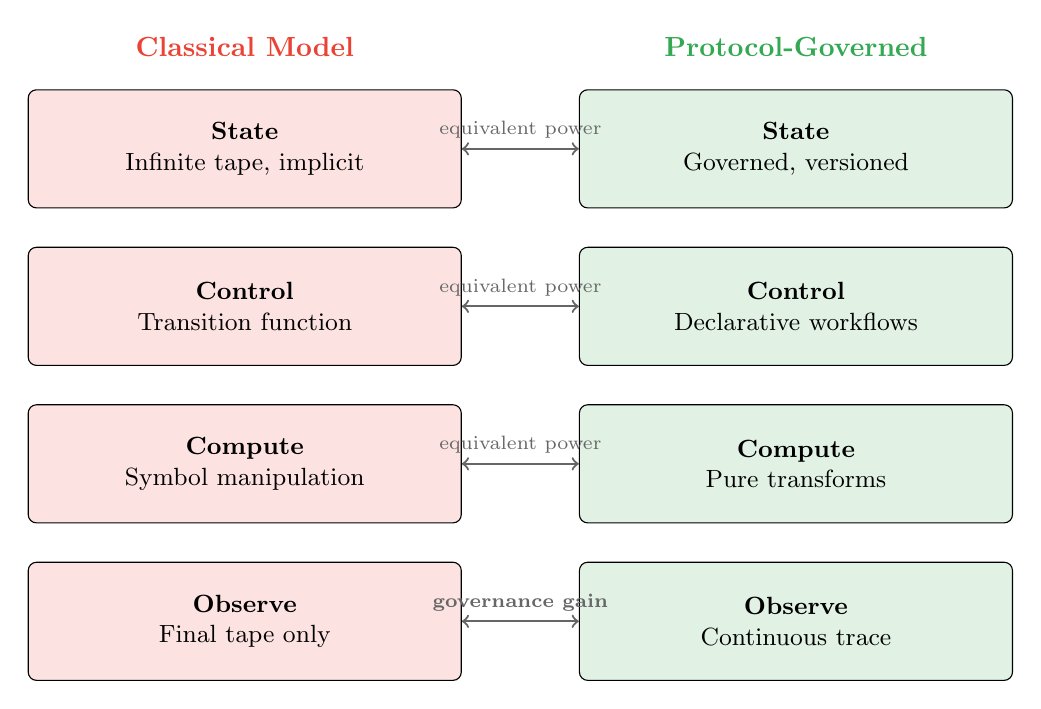
\begin{tikzpicture}[
    primbox/.style={
        rectangle, draw, rounded corners=3pt,
        minimum width=5.5cm, minimum height=1.5cm,
        align=center, font=\small
    },
    arrow/.style={->, thick, black!60}
]

% Classical side
\node[primbox, fill=classicalcolor!15] (cstate) at (-3.5, 6) {
    \textbf{State}\\
    Infinite tape, implicit
};
\node[primbox, fill=classicalcolor!15] (ccontrol) at (-3.5, 4) {
    \textbf{Control}\\
    Transition function
};
\node[primbox, fill=classicalcolor!15] (ccompute) at (-3.5, 2) {
    \textbf{Compute}\\
    Symbol manipulation
};
\node[primbox, fill=classicalcolor!15] (cobserve) at (-3.5, 0) {
    \textbf{Observe}\\
    Final tape only
};

% Protocol-governed side
\node[primbox, fill=governedcolor!15] (pstate) at (3.5, 6) {
    \textbf{State}\\
    Governed, versioned
};
\node[primbox, fill=governedcolor!15] (pcontrol) at (3.5, 4) {
    \textbf{Control}\\
    Declarative workflows
};
\node[primbox, fill=governedcolor!15] (pcompute) at (3.5, 2) {
    \textbf{Compute}\\
    Pure transforms
};
\node[primbox, fill=governedcolor!15] (pobserve) at (3.5, 0) {
    \textbf{Observe}\\
    Continuous trace
};

% Labels
\node[font=\bfseries, text=classicalcolor] at (-3.5, 7.3) {Classical Model};
\node[font=\bfseries, text=governedcolor] at (3.5, 7.3) {Protocol-Governed};

% Equivalence arrows
\draw[arrow, <->] (cstate) -- (pstate) node[midway, above, font=\scriptsize] {equivalent power};
\draw[arrow, <->] (ccontrol) -- (pcontrol) node[midway, above, font=\scriptsize] {equivalent power};
\draw[arrow, <->] (ccompute) -- (pcompute) node[midway, above, font=\scriptsize] {equivalent power};
\draw[arrow, <->] (cobserve) -- (pobserve) node[midway, above, font=\scriptsize] {\textbf{governance gain}};

\end{tikzpicture}
\caption{Computational primitives: classical vs.\ protocol-governed. Both models achieve equivalent computational power; the protocol-governed model adds intrinsic observability.}
\label{fig:primitives}
\end{figure}


%% ============================================================
%% SECTION 5: CONDITIONS FOR TURING COMPLETENESS
%% ============================================================

\section{Conditions for Turing Completeness Under Governance}
\label{sec:conditions}

\subsection{Minimal Requirements for Universal Computation}

The Church-Turing thesis establishes that any system capable of simulating a Turing machine can compute any computable function \citep{sipser2012introduction}. The minimal requirements for such simulation are well-characterized:

\begin{enumerate}[nosep]
    \item \textbf{Unbounded Storage:} The system must be capable of storing an arbitrarily large amount of symbolic information.
    \item \textbf{Conditional Branching:} The system must be capable of executing different operations based on stored state.
    \item \textbf{Unbounded Iteration:} The system must be capable of repeating operations an arbitrary number of times.
\end{enumerate}

These requirements are \emph{necessary and sufficient}. Any system satisfying them can simulate a Turing machine; any system failing to satisfy them cannot \citep{hopcroft2006automata}.

\subsection{How Protocol-Governed Systems Satisfy These Requirements}

Protocol-governed systems satisfy the requirements for Turing completeness through their architectural primitives:

\textbf{Unbounded Storage.} Governed state containers (capability side effects) provide unbounded symbolic storage. While any physical implementation has finite bounds, the \emph{architectural model} places no limit on state capacity. A governed storage contract can hold an arbitrarily large data structure, just as a Turing tape can hold an arbitrarily long symbol sequence.

\textbf{Conditional Branching.} Workflow orchestration provides declarative conditional branching. Workflow nodes may route to different successors based on state conditions. This is semantically equivalent to the Turing machine's transition function: current state determines next operation.

\textbf{Unbounded Iteration.} Lawful re-invocation enables unbounded iteration. Lawful re-invocation is semantically equivalent to recursion, not syntactic recursion. A workflow may invoke operations that, through protocol-governed recursion, repeat an arbitrary number of times. Unlike imperative loops, this iteration occurs through declared invocation paths---but the computational power is equivalent.

\subsection{Why Governance Does Not Reduce Expressiveness}

A potential objection: does constitutional constraint reduce computational power? If behaviors are vocabulary-bounded, can all computable functions be expressed?

The answer is no---governance does not reduce expressiveness---for a fundamental reason: \emph{governance constrains mechanism, not outcome}. A governed system may compute any function that an ungoverned system can compute. The difference is in how computation is achieved:

\begin{itemize}[nosep]
    \item In ungoverned systems, computation proceeds through arbitrary state mutation and control flow.
    \item In governed systems, computation proceeds through declared artifacts, explicit transitions, and traced execution.
\end{itemize}

The space of computable outcomes is identical. The space of permissible mechanisms is constrained. This is precisely the architectural property we seek: universal expressiveness with bounded mechanism.

\begin{proposition}[Governance-Expressiveness Independence]
Let $\mathcal{C}$ be the class of computable functions. Let $\mathcal{P}$ be a protocol-governed system satisfying the conditions of Section~\ref{sec:conditions}. Then for any $f \in \mathcal{C}$, there exists a protocol specification $\pi$ such that $\mathcal{P}$ executing $\pi$ computes $f$.
\end{proposition}

The proposition asserts that governance does not exclude any computable function from the system's expressive range.


%% ============================================================
%% SECTION 6: COMPARISON TO CLASSICAL TURING MACHINES
%% ============================================================

\section{Comparison to Classical Turing Machines}
\label{sec:comparison}

The following comparison illuminates the architectural distinction between classical and protocol-governed computation:

\begin{table}[h]
\centering
\caption{Architectural comparison: Classical Turing Machine vs.\ Protocol-Governed System.}
\label{tab:comparison}
\begin{tabular}{@{}lll@{}}
\toprule
\textbf{Aspect} & \textbf{Classical TM} & \textbf{Protocol-Governed} \\
\midrule
State & Infinite tape, implicit & Governed containers, explicit \\
Control & Transition function & Declarative workflow law \\
Mutation & Implicit, unconstrained & Explicit, traced \\
Semantics & Inferred from execution & Declared in artifacts \\
Auditability & None (external only) & Structural (trace-based) \\
Governance & None & Constitutional \\
Replaceability & Implementation-bound & Engine-independent \\
Authority & Absent & First-class \\
\bottomrule
\end{tabular}
\end{table}

The comparison reveals that protocol-governed systems add governance dimensions absent from classical models while preserving computational universality. This is not a trade-off but an augmentation: governed systems can do everything classical systems can do, plus provide auditability, authority, and semantic stability.

\subsection{The Governance Invariant}

We can state the relationship formally:

\begin{theorem}[Informal]
A protocol-governed system with unbounded governed storage, conditional workflow branching, and lawful re-invocation can simulate any Turing machine while maintaining complete execution traceability.
\end{theorem}

The significance is that traceability is not purchased at the cost of expressiveness. The two properties are orthogonal: one concerns \emph{what} can be computed; the other concerns \emph{how} computation is witnessed.

\subsection{Why This Is Not Merely a Turing Machine With Logging}

A superficial reading might dismiss protocol-governed computation as ``a Turing machine with logging.'' This misses the architectural distinction:

In a ``Turing machine with logging,'' logging is an external observation of an unconstrained computation. The machine computes as it pleases; the log records what happened. Logging does not constrain the machine, and the machine's behavior is defined independently of logging.

In a protocol-governed system, traceability is \emph{constitutive} of computation. Execution \emph{cannot occur} except through governed pathways that produce traces. There is no ``underlying computation'' that is separately logged. The computation \emph{is} the traced execution of declared behavior.

This distinction matters for governance. A logged Turing machine can be audited, but auditing is external and after-the-fact. A protocol-governed system is governed intrinsically---behavior that cannot be declared cannot be computed.

% ---- FIGURE 2: TURING MACHINE VS PROTOCOL-GOVERNED ----
\begin{figure}[H]
\centering
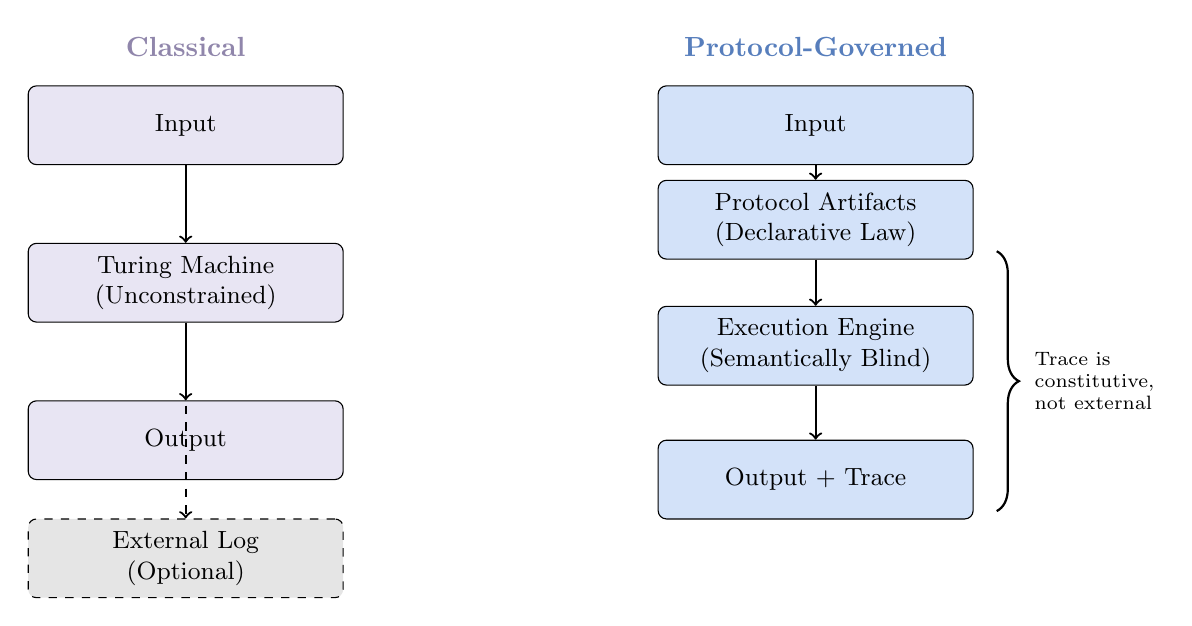
\begin{tikzpicture}[
    box/.style={
        rectangle, draw, rounded corners=3pt,
        minimum width=4cm, minimum height=1cm,
        align=center, font=\small
    },
    arrow/.style={->, thick}
]

% Classical TM side
\node[box, fill=turingcolor!30] (tm_input) at (-4, 4) {Input};
\node[box, fill=turingcolor!30] (tm_machine) at (-4, 2) {Turing Machine\\(Unconstrained)};
\node[box, fill=turingcolor!30] (tm_output) at (-4, 0) {Output};

\draw[arrow] (tm_input) -- (tm_machine);
\draw[arrow] (tm_machine) -- (tm_output);

% External logging (dashed)
\node[box, fill=gray!20, dashed] (tm_log) at (-4, -1.5) {External Log\\(Optional)};
\draw[arrow, dashed] (tm_machine) -- (tm_log);

% Protocol-governed side
\node[box, fill=protocolcolor!30] (pg_input) at (4, 4) {Input};
\node[box, fill=protocolcolor!30] (pg_protocol) at (4, 2.8) {Protocol Artifacts\\(Declarative Law)};
\node[box, fill=protocolcolor!30] (pg_engine) at (4, 1.2) {Execution Engine\\(Semantically Blind)};
\node[box, fill=protocolcolor!30] (pg_output) at (4, -0.5) {Output + Trace};

\draw[arrow] (pg_input) -- (pg_protocol);
\draw[arrow] (pg_protocol) -- (pg_engine);
\draw[arrow] (pg_engine) -- (pg_output);

% Labels
\node[font=\bfseries, text=turingcolor!80!black] at (-4, 5) {Classical};
\node[font=\bfseries, text=protocolcolor!80!black] at (4, 5) {Protocol-Governed};

% Key distinction annotation
\draw[decorate, decoration={brace, amplitude=8pt, mirror}, thick]
    (6.3, -0.9) -- (6.3, 2.4) node[midway, right=10pt, font=\scriptsize, align=left] {Trace is\\constitutive,\\not external};

\end{tikzpicture}
\caption{Architectural distinction: Classical Turing machines compute with optional external logging. Protocol-governed systems produce traces as an intrinsic property of execution.}
\label{fig:tm-vs-pg}
\end{figure}


%% ============================================================
%% SECTION 7: IS CONSTRAINED COMPUTATION AN ANTI-PATTERN?
%% ============================================================

\section{Is Constrained Computation an Anti-Pattern?}
\label{sec:antipattern}

\subsection{The Objection: Constraints Limit Power}

A reasonable objection arises: constraints are generally understood to limit capability. If we constrain how computation occurs, do we not limit what computation can achieve?

This objection conflates two senses of ``limit'':

\begin{enumerate}[nosep]
    \item \textbf{Outcome Limitation:} Reducing the set of computable results
    \item \textbf{Mechanism Limitation:} Reducing the set of permissible computational paths
\end{enumerate}

Protocol governance imposes mechanism limitation, not outcome limitation. Any computable outcome remains achievable; the paths to that outcome are disciplined.

Consider an analogy: traffic laws constrain how vehicles may travel, but they do not limit where vehicles can go. A driver obeying traffic laws can reach any destination a lawless driver can reach. The journey is different; the destination space is unchanged.

\subsection{Why Constraint Is a Feature}

In the context of governed systems, mechanism limitation is precisely what is desired. The goal is not to prevent any particular computation but to ensure that all computation occurs through auditable, authorized, traceable channels.

Consider the alternative: a system with unconstrained computational power that can produce any side effect, invoke any external service, and modify any state without governance. Such a system is maximally powerful and minimally governable. Its behavior cannot be predicted from its artifacts, verified through its traces, or constrained by its architecture.

Protocol governance trades mechanism freedom for behavioral clarity. This is the right trade-off for systems requiring:

\begin{itemize}[nosep]
    \item Long-term auditability
    \item Regulatory compliance
    \item Multi-stakeholder governance
    \item AI-assisted development with preserved meaning
    \item Safety-critical operation
\end{itemize}

\subsection{Expressiveness Through Composition}

Protocol-governed systems achieve expressiveness through composition rather than primitive complexity. Simple, well-governed primitives combine to produce complex behavior. The composition itself is declared, versioned, and governed.

This compositional approach offers advantages beyond governance:

\begin{itemize}[nosep]
    \item \textbf{Testability:} Primitive transforms are independently testable
    \item \textbf{Reusability:} Governed primitives compose across workflows
    \item \textbf{Evolvability:} New behaviors emerge from novel compositions of stable primitives
    \item \textbf{Comprehensibility:} Complex behavior decomposes into understood components
\end{itemize}


%% ============================================================
%% SECTION 8: IMPLICATIONS FOR THE AI ERA
%% ============================================================

\section{Implications for the AI Era}
\label{sec:ai-era}

\subsection{AI as Execution Generator, Not Law Author}

The emergence of AI-assisted software development creates both opportunity and risk \citep{chen2021evaluating,github2023copilot}. AI excels at generating implementation code---the mechanical translation of behavioral intent into executable instructions. AI struggles to preserve behavioral semantics when refactoring, optimizing, or extending existing systems \citep{pearce2022asleep}.

Protocol-governed architecture aligns with AI capabilities. AI may generate, optimize, and replace execution engines without constraint, provided the engines conform to protocol specifications. Behavioral equivalence is verified mechanically through trace comparison. AI becomes an execution generator, not a law author.

The protocol---the declarative specification of what the system does---remains under human governance. AI contributes implementation; humans govern behavior. This division of labor exploits AI strengths while mitigating AI risks.

\subsection{Semantic Drift Resistance}

Semantic drift---the gradual divergence between intended and actual system behavior---is endemic to imperative software \citep{parnas1972criteria}. Each modification risks subtle behavioral change. Over time, systems become inscrutably different from their original specifications.

Protocol-governed systems resist semantic drift structurally. Behavioral specification exists independently of implementation. Execution engines may evolve, optimize, or be replaced, but the behavioral specification remains authoritative. Conformance verification ensures that implementation evolution does not introduce semantic divergence.

This property is essential for AI-accelerated development. When AI modifies implementation at velocities exceeding human audit capacity, the only viable governance strategy is specification-based verification. If behavior is defined by implementation, AI modification is ungovernable. If behavior is defined by protocol, AI modification is verifiable.

\subsection{The Governance Imperative}

We can now state the core argument: in AI-accelerated software environments, governance must be architectural, not procedural.

Procedural governance---code review, testing, documentation---scales with human velocity. As AI increases implementation velocity, procedural governance becomes the bottleneck. Review backlogs grow; testing coverage declines; documentation diverges from implementation.

Architectural governance---specification-based verification, trace-based conformance, vocabulary-bounded behavior---scales with machine velocity. Conformance verification is automated. Behavioral equivalence is mechanically proven. Semantic drift is structurally prevented.

Protocol-governed architecture provides architectural governance. It is not merely a software pattern but a governance strategy adapted to the realities of AI-accelerated development.


%% ============================================================
%% SECTION 9: RELATED WORK
%% ============================================================

\section{Related Work}
\label{sec:related}

\subsection{Turing Machines and Computational Theory}

The foundation of computability theory rests on Turing's seminal work establishing the limits of mechanical calculation \citep{turing1936computable}. Church's lambda calculus provides an equivalent formulation through function abstraction \citep{church1936unsolvable}. Subsequent developments---recursive function theory \citep{rogers1987theory}, register machines \citep{shepherdson1963computability}---provided alternative characterizations of the same computational class. These works characterize \emph{what} can be computed but do not address \emph{how} computation should be governed.

\subsection{Formal Specification Languages}

TLA+ enables rigorous behavioral specification through temporal logic \citep{lamport2002specifying}. Alloy provides lightweight formal methods through relational modeling \citep{jackson2012software}. Z and VDM offer mathematical notation for software specification \citep{spivey1989z}. These approaches share protocol-governed architecture's emphasis on declarative behavioral specification.

The distinction is execution authority. Formal specification languages traditionally separate specification from implementation: the specification is verified, then translated to code, then executed. Protocol-governed architecture maintains specification authority through execution. The specification is not translated but interpreted; it remains authoritative throughout the system lifecycle.

\subsection{Workflow Systems}

Workflow engines based on Petri nets \citep{vanderaalst2003workflow} and BPMN \citep{omg2011bpmn} provide orchestration governance: they control the sequencing and routing of computational steps. However, workflow engines typically delegate semantic authority to the code invoked at each step. The workflow declares \emph{when} operations execute; the operations themselves are governed (or not) independently.

Protocol-governed systems extend governance from orchestration to semantics. Capability contracts govern not just when operations execute but what operations are permitted, what inputs they accept, what outputs they produce, and what side effects they may cause.

\subsection{Model-Driven Architecture}

The OMG's Model-Driven Architecture (MDA) separates platform-independent models from platform-specific implementations \citep{omg2014mda}. Models are transformed into code, which is then compiled and executed.

The distinction from protocol governance is authority persistence. In MDA, the model generates code; the code becomes authoritative. In protocol-governed systems, the specification remains authoritative through execution. This difference is subtle but consequential: protocol-governed systems can verify behavioral equivalence across engine implementations because the specification, not the code, defines correct behavior.

\subsection{Capability-Based Security}

Capability-based security systems constrain computational authority through unforgeable tokens \citep{dennis1966multiprogrammed,miller2003capability}. A process may only perform operations for which it holds capabilities. This approach shares protocol governance's emphasis on explicit authority.

Protocol-governed systems apply capability principles to behavioral governance, not just resource access. Capability contracts govern not only which resources a computation may access but what behaviors it may exhibit.


%% ============================================================
%% SECTION 10: LIMITATIONS AND NON-GOALS
%% ============================================================

\section{Limitations and Non-Goals}
\label{sec:limitations}

\subsection{What This Paper Does Not Claim}

\textbf{This is not a programming language proposal.} Protocol-governed computation is an architectural model, not a language design. The artifacts that declare behavior may be authored in various notations; the architecture is independent of authoring syntax.

\textbf{This is not a new complexity class.} Protocol-governed systems are Turing complete. They compute the same class of functions as classical models. The contribution is architectural, not computational-theoretic.

\textbf{This is not a replacement for low-level systems programming.} Operating systems, device drivers, and performance-critical infrastructure may require implementation patterns that protocol governance does not address. The architecture is optimized for business logic, compliance-critical systems, and long-lived applications.

\subsection{Appropriate Domains}

Protocol-governed computation is optimized for systems characterized by:

\begin{itemize}[nosep]
    \item Long operational lifetimes (years to decades)
    \item Multi-stakeholder governance requirements
    \item Regulatory or compliance obligations
    \item Behavioral auditability mandates
    \item AI-assisted development with semantic preservation needs
    \item Safety-critical or high-assurance domains
\end{itemize}

It is less applicable to short-lived scripts and utilities, performance-critical inner loops, systems requiring unconstrained low-level access, and exploratory or prototyping contexts.

\subsection{Governance Overhead}

Protocol governance imposes upfront costs. Behavioral specification requires explicit declaration of workflows, contracts, and authority. This overhead may not be justified for systems where governance is not a concern.

The architecture does not claim universal applicability. It claims that for systems where governance matters, architectural governance is superior to procedural governance, and constitutional constraint is compatible with computational universality.


%% ============================================================
%% SECTION 11: CONCLUSION
%% ============================================================

\section{Conclusion}
\label{sec:conclusion}

The classical theory of computation answered the question ``What can be computed?'' Protocol-governed computation addresses a different question: ``What can be computed while remaining governed?''

This paper has demonstrated that the answer is: anything. Turing completeness is achievable within constitutional constraint. Universal computation does not require unconstrained execution.

The key insights are:

\begin{enumerate}[nosep]
    \item \textbf{Governance is architectural, not external.} Constrained computation is not computation-with-governance-added but a different computational architecture in which governance is constitutive.

    \item \textbf{Constraint does not reduce expressiveness.} The space of computable outcomes is unchanged. The space of permissible mechanisms is disciplined. Mechanism constraint enables governance without outcome limitation.

    \item \textbf{Traceability is intrinsic, not optional.} Execution produces evidence. This evidence enables verification, audit, and behavioral equivalence proof---capabilities absent from classical computational models.

    \item \textbf{Implementation is replaceable.} Execution engines are interchangeable. Behavioral equivalence is verified through trace comparison. AI may generate engines; humans govern behavior.
\end{enumerate}

For the AI era, this reframing is essential. When AI generates the majority of production code, behavioral governance cannot rely on code inspection. It must rely on specification authority---declarative artifacts that define what systems do, independent of how they do it.

Protocol-governed computation provides that foundation. It preserves universal expressiveness while enforcing constitutional constraint. It enables computation that is simultaneously powerful and governable.

This is not a theoretical curiosity. It is an architectural necessity for systems that must remain auditable, deterministic, and semantically stable as implementation velocity accelerates beyond human governance capacity.

Computation becomes a governed act---not an accidental side effect.


%% ============================================================
%% LICENSE, AUTHOR, REFERENCES
%% ============================================================

\section*{License and Use}

This work is licensed under the Creative Commons Attribution-NonCommercial-NoDerivatives 4.0 International License (CC BY-NC-ND 4.0).

You are free to share and redistribute this material in any medium or format, provided that: appropriate credit is given to the author, the material is not used for commercial purposes, and the material is not modified, transformed, or built upon.

The paper does not grant rights to implement patented methods, systems, or workflows that may be covered by pending or future patent claims.

For licensing inquiries or permissions beyond the scope of this license, contact the author.

\section*{Author Information}

\noindent Bachi (aka Bhash Ganti)\\
Contact: \texttt{bachi.bachi@myyahoo.com}

\noindent\textbf{Conflict of Interest:} The author is developing commercial implementations of the described architecture.

\bibliographystyle{plainnat}

\begin{thebibliography}{99}

\bibitem[Bachi(2026a)]{bachi2026protocol}
Bachi aka Bhash Ganti (2026a).
\newblock Protocol-Governed Systems: An Architectural Foundation for the AI Era.
\newblock Zenodo Working Paper.
\newblock DOI: \url{https://doi.org/10.5281/zenodo.18715516}.

\bibitem[Barendregt(1984)]{barendregt1984lambda}
Barendregt, H.P. (1984).
\newblock \emph{The Lambda Calculus: Its Syntax and Semantics}.
\newblock North-Holland, revised edition.

\bibitem[Chen et~al.(2021)]{chen2021evaluating}
Chen, M., Tworek, J., Jun, H., Yuan, Q., Pinto, H.P.O., Kaplan, J., et~al. (2021).
\newblock Evaluating large language models trained on code.
\newblock \emph{arXiv preprint arXiv:2107.03374}.

\bibitem[Church(1936)]{church1936unsolvable}
Church, A. (1936).
\newblock An unsolvable problem of elementary number theory.
\newblock \emph{American Journal of Mathematics}, 58(2):345--363.

\bibitem[Dennis and Van~Horn(1966)]{dennis1966multiprogrammed}
Dennis, J.B. and Van~Horn, E.C. (1966).
\newblock Programming semantics for multiprogrammed computations.
\newblock \emph{Communications of the ACM}, 9(3):143--155.

\bibitem[GitHub(2023)]{github2023copilot}
GitHub (2023).
\newblock GitHub Copilot research recitation.
\newblock Technical report, GitHub.

\bibitem[Hopcroft et~al.(2006)]{hopcroft2006automata}
Hopcroft, J.E., Motwani, R., and Ullman, J.D. (2006).
\newblock \emph{Introduction to Automata Theory, Languages, and Computation}.
\newblock Addison-Wesley, 3rd edition.

\bibitem[Jackson(2012)]{jackson2012software}
Jackson, D. (2012).
\newblock \emph{Software Abstractions: Logic, Language, and Analysis}.
\newblock MIT Press, revised edition.

\bibitem[Lamport(2002)]{lamport2002specifying}
Lamport, L. (2002).
\newblock \emph{Specifying Systems: The TLA+ Language and Tools for Hardware and Software Engineers}.
\newblock Addison-Wesley.

\bibitem[Miller et~al.(2003)]{miller2003capability}
Miller, M.S., Yee, K.-P., and Shapiro, J. (2003).
\newblock Capability myths demolished.
\newblock Technical report, Combex, Inc.

\bibitem[Minsky(1967)]{minsky1967computation}
Minsky, M.L. (1967).
\newblock \emph{Computation: Finite and Infinite Machines}.
\newblock Prentice-Hall.

\bibitem[Object Management Group(2011)]{omg2011bpmn}
Object Management Group (2011).
\newblock Business process model and notation (BPMN) version 2.0.
\newblock OMG Standard.

\bibitem[Object Management Group(2014)]{omg2014mda}
Object Management Group (2014).
\newblock Model driven architecture (MDA) guide revision 2.0.
\newblock OMG Document ormsc/14-06-01.

\bibitem[Parnas(1972)]{parnas1972criteria}
Parnas, D.L. (1972).
\newblock On the criteria to be used in decomposing systems into modules.
\newblock \emph{Communications of the ACM}, 15(12):1053--1058.

\bibitem[Pearce et~al.(2022)]{pearce2022asleep}
Pearce, H., Ahmad, B., Tan, B., Dolan-Gavitt, B., and Karri, R. (2022).
\newblock Asleep at the keyboard? Assessing the security of GitHub Copilot's code contributions.
\newblock In \emph{IEEE Symposium on Security and Privacy}, pages 754--768.

\bibitem[Plotkin(1981)]{plotkin1981structural}
Plotkin, G.D. (1981).
\newblock A structural approach to operational semantics.
\newblock Technical Report DAIMI FN-19, Computer Science Department, Aarhus University.

\bibitem[Rogers(1987)]{rogers1987theory}
Rogers, H. (1987).
\newblock \emph{Theory of Recursive Functions and Effective Computability}.
\newblock MIT Press.

\bibitem[Scott and Strachey(1971)]{scott1971semantics}
Scott, D. and Strachey, C. (1971).
\newblock Toward a mathematical semantics for computer languages.
\newblock \emph{Proceedings of the Symposium on Computers and Automata}, pages 19--46.

\bibitem[Shepherdson and Sturgis(1963)]{shepherdson1963computability}
Shepherdson, J.C. and Sturgis, H.E. (1963).
\newblock Computability of recursive functions.
\newblock \emph{Journal of the ACM}, 10(2):217--255.

\bibitem[Sipser(2012)]{sipser2012introduction}
Sipser, M. (2012).
\newblock \emph{Introduction to the Theory of Computation}.
\newblock Cengage Learning, 3rd edition.

\bibitem[Spivey(1989)]{spivey1989z}
Spivey, J.M. (1989).
\newblock \emph{The Z Notation: A Reference Manual}.
\newblock Prentice Hall.

\bibitem[Turing(1936)]{turing1936computable}
Turing, A.M. (1936).
\newblock On computable numbers, with an application to the Entscheidungsproblem.
\newblock \emph{Proceedings of the London Mathematical Society}, 2(42):230--265.

\bibitem[van~der Aalst et~al.(2003)]{vanderaalst2003workflow}
van~der Aalst, W.M.P., ter~Hofstede, A.H.M., Kiepuszewski, B., and Barros, A.P. (2003).
\newblock Workflow patterns.
\newblock \emph{Distributed and Parallel Databases}, 14(1):5--51.

\end{thebibliography}

\end{document}
